\documentclass[emulatestandardclasses]{scrartcl}
\usepackage{graphicx}
\usepackage{color}
\usepackage[ngerman]{babel}
\usepackage{hyperref}
\usepackage{fullpage}
\usepackage[utf8]{inputenc}
\usepackage{calc} 
\usepackage{enumitem}
\usepackage{titlesec}
\newcommand{\todo}[1]{\textcolor{red}{TODO: #1}\PackageWarning{TODO:}{#1!}}
\date{\vspace{-3ex}}
\begin{document}

\title{
	\includegraphics*[width=0.75\textwidth]{ErstesSem/images/hu_logo.png}\\
	\vspace{24pt}
	Die Erfahrung der Realität\\durch Widerstand}
\subtitle{\vspace{10pt}Proseminar WS 17/18\\
          Matthias Schlo"sberger\\
          Philosophisches Institut I \\ 
          Humboldt Universit"at zu Berlin}
\author{Lennard Wolf\\
        \small{\href{mailto:lennard.wolf@student.hu-berlin.de}{lennard.wolf@student.hu-berlin.de}}}
\maketitle
\begin{abstract}
Häufig wird Erkenntnistheorie als Versuch der Rechtfertigung von Erkenntnis betrieben. Dass es möglich ist, von der Rechtfertigung einer Erkenntnis zu sprechen, verweist auf ein Problem, das vor allen Fragen der Rechtfertigung geklärt werden sollte. Bevor eine Erkenntnis gerechtfertigt werden kann, muss das in der Erkenntnis Erkannte erfahren werden. Dies, so die Arbeitshypothese des Seminars, gilt auch und insbesondere für die Erfahrung von Realität.
Eine mögliche Antwort auf die Frage, wie die Erfahrung der Realität gemacht wird, lautet: durch die Erfahrung der Widerständigkeit von etwas (der Welt, des Psychischen, des Physischen, des Anderen etc.). Ziel des Seminars ist es, diese Antwort bei einigen für dieses Thema klassischen Autoren zu untersuchen. Besonders wichtig wird es sein, einen klaren Begriff des Widerstands zu entwickeln, der an vielen verschiedenen Phänomenen erläutert werden kann.

\end{abstract}
\newpage

\tableofcontents
\listoffigures
\newpage


\section{Einf"uhrung\\(19.10.17)}

\subsection{Einf"uhrung}


\newpage
%\section{"Uber den Professor}
%Matthias Schlo"sberger ist Heisenbergstipendiat der Deutschen Forschungsgemeinschaft
%an der Humboldt Universit"at zu Berlin mit dem Forschungsprojekt "`Die Erfahrung der Realit"at durch Widerstand"'.
%
%\begin{figure}[h]
%	\centering
%	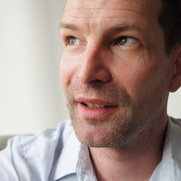
\includegraphics[width=0.3\textwidth]{images/Matthias_Schlossberger.png}
%	\caption{Matthias Schlo"sberger}
%	\label{fig:MS}
%\end{figure}


%\begin{figure}[h]
%	\centering
%	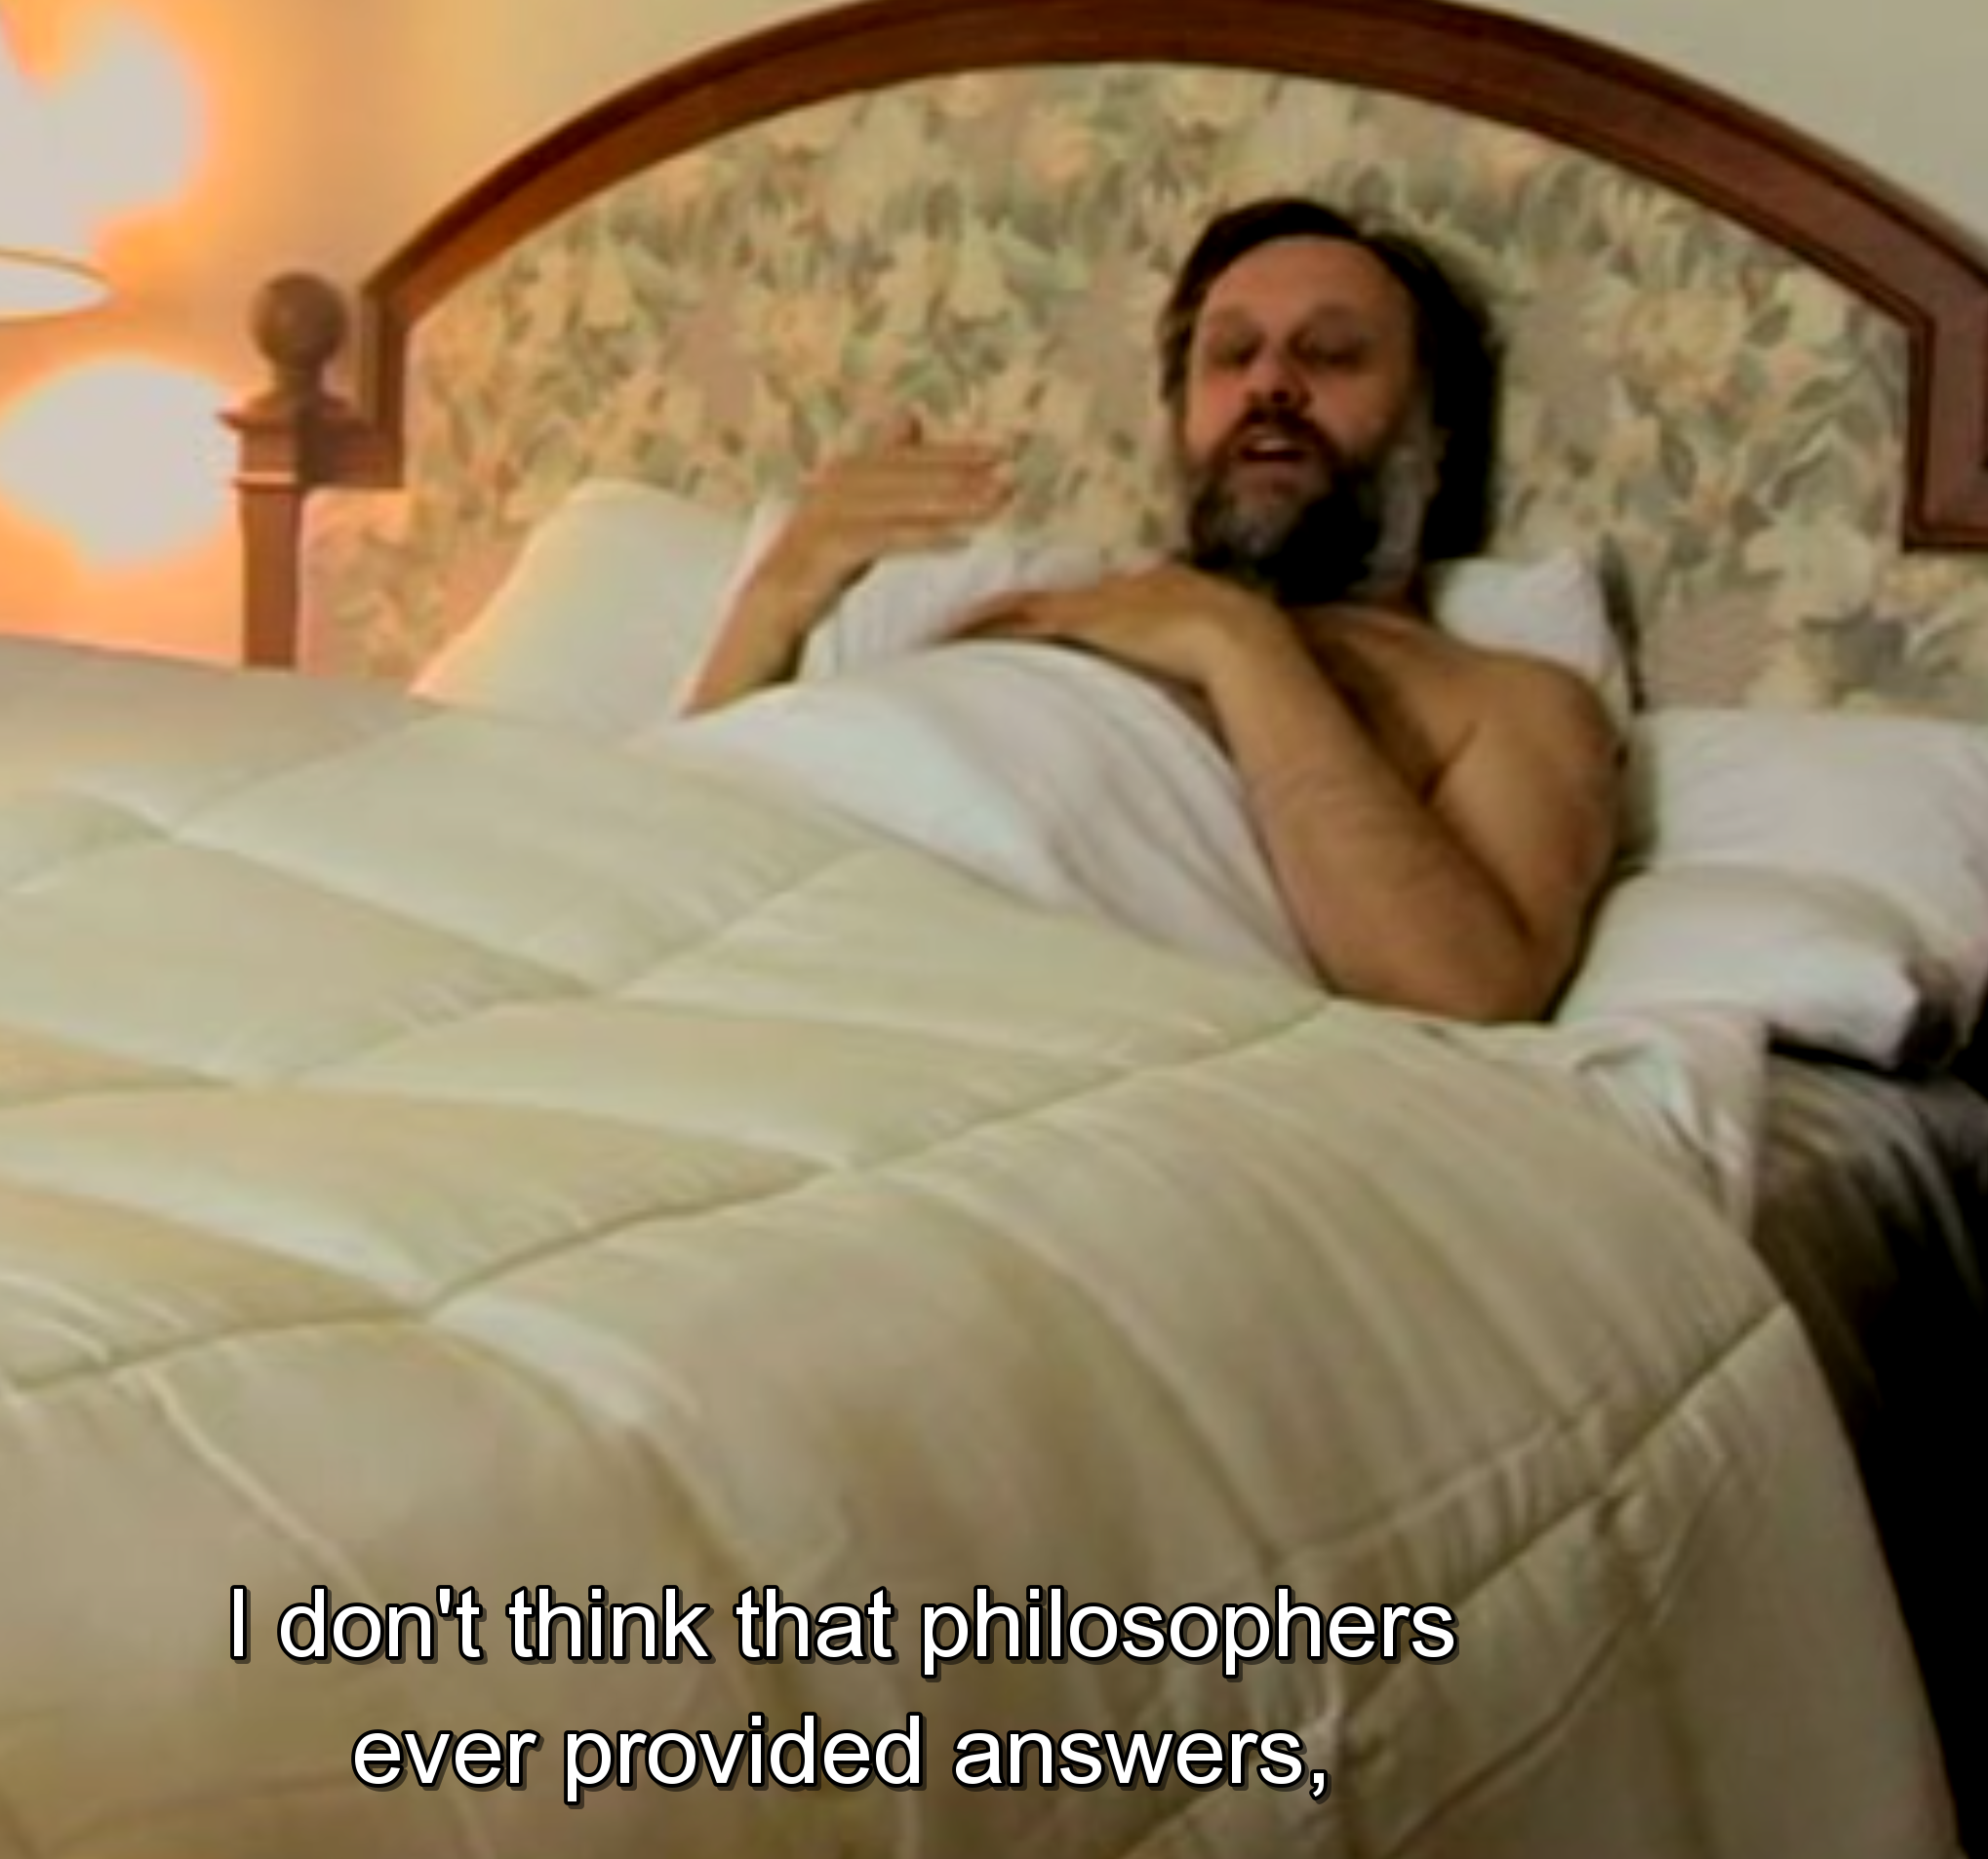
\includegraphics[width=0.5\textwidth]{images/template.png}
%	\caption{Template Bild}
%	\label{fig:template}
%\end{figure}

\end{document}
